\documentclass{article}

% Language setting
% Replace `english' with e.g. `spanish' to change the document language
\usepackage{polski}
\usepackage[utf8]{inputenc}

% Set page size and margins
% Replace `letterpaper' with`a4paper' for UK/EU standard size
\usepackage[letterpaper,top=2cm,bottom=2cm,left=3cm,right=3cm,marginparwidth=1.75cm]{geometry}

% Useful packages
\usepackage{amsmath}
\usepackage{graphicx}
\usepackage[colorlinks=true, allcolors=blue]{hyperref}

\title{Zaawansowane algorytmy i struktury danych \\ Algorytm kompresji Lempel-Ziv}
\author{Dawid Bitner}

\begin{document}
\maketitle

\section{Wstęp}
Algorytmy z rodziny Lempel-Ziv, głównie takie jak \textit{LZ77} czy \textit{LZ78} są algorytmami kompresji bezstratnej. Kompresję bezstratną możemy zdefiniować jako kodowanie bezstratne w taki sposób, aby minimalizować długość komunikatu po zakodowaniu. Kodem jest zbiór słów kodowych przyporządkowanych ciągom symboli alfabetu źródła bądź też poszczególnym  symbolom  tego  alfabetu.  Natomiast słowa  kodowe  to  ciągi  symboli  pewnego  alfabetu,  który  będzie  określany  mianem  alfabetu  kodu. Algorytmy takie nie nadają się jednak do kompresji wszystkich typów informacji. Nie znajdą zastosowania m.in.: w kompresowaniu strumienia liczb losowych i pseudolosowych.

\section{Opis historyczny (geneza)}
 W roku 1977 dwaj izarealscy naukowcy - informatycy: Abraham Lempel i Jacob Ziv opublikowali przełomowy algorytm kompresji bezstratnej, który swoją nazwę zawdzięcza pierwszym literom nazwiska twórców i dacie jego opracowania - czyli \textit{LZ77}. Był to algorytm przełomowy, ponieważ jako pierwszy algorytm wykorzystywał słownik do kompresji danych. \textit{LZ77} używa słownika dynamicznego - nazywanego również często oknem przesuwnym. Rok później, w 1978, ta sama para naukowców opublikowała kolejny algorytm - \textit{LZ78}. Algorytm ten również używa słownika, jednak w przeciwieństwie do \textit{LZ77}, algorytm ten analizuje dane wejsciowe i generuje statyczny słownik zamiast generować go dynamicznie.
 Zarówno algorytmy \textit{LZ77}, jak i \textit{LZ78} szybko zyskały na popularności - powstały ich modyfikacje jak np.: \textit{LZW}. \\
Ciekawostką jest, że większość powszechnie stosowanych algorytmów wywodzi się z algorytmu \textit{LZ77}. Nie wynika to z przewagi technicznej tego algorytmu, ale z tego że algorytmy \textit{LZ78} zostały obciążone patentami po tym, jak pochodny algorytm \textit{LZW} został opatentowany w 1984 roku i autor patentu zaczął pozywać dostawców oprogramowania, administratorów serwerów, a nawet użytkowników końcowych za używanie formatu GIF bez licencji.

\begin{figure}[h!]
\centering {
\hfill
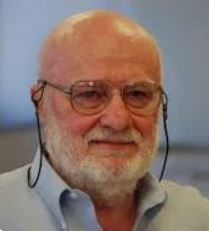
\includegraphics[height=5cm]{img/abraham_lempel.JPG}
\hfill
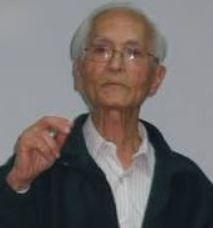
\includegraphics[height=5cm]{img/jacob_ziv.JPG}
\hfill
}
\caption{Twórcy algorytmu: Abraham Lempel oraz Jacob Ziv.}
\label{fig:mobile_test_code_view}
\end{figure}

\section{Algorytmy}
\subsection{LZ77}
W kodowaniu \textit{LZ77} przechowuje się bufor (tzw. okno) będące połączeniem bufora słownikowego który zawiera określoną liczbę ostatnio kodowanych symboli i bufora kodowania z pewną liczbą symboli, które dopiero mają zostać w kolejnym kroku poddane kodowaniu. Rozpoczynając proces kodowania wypełniamy bufor słownikowy powtórzeniami pierwszego symbolu zawartości ciągu kodowanego, a bufor kodowania przedrostkiem kodowanego komunikatu, o długości równej długości bufora kodowania. Następnie cyklicznie wyszukujemy najdłuższy przedrostek $f$ bufora  kodowania  w  oknie.  Poszukiwania rozpoczynamy od końca bufora słownikowego po lewej stronie i przesuwamy się w prawo. Znalezione w ten sposób  dopasowanie $f$ może mieć długość większą od długości bufora słownikowego, nie większą jednak od długości okna. Po znalezieniu $f$ wyprowadzamy trójkę $<d, l, c>$, gdzie $d$ oznacza pozycję $f$ w buforze słownikowym, $l$ to długość $f$, a $c$ to symbol, dla którego $f$ jest przedrostkiem  w  oknie, czyli pierwszy symbol znajdujący się w buforze kodowania za $f$. Po  wyprowadzeniu  trójki  $<d, l, c>$  zawartość  okna  przesuwamy  o  $l$  pozycji  w  lewo,  wprowadzając  jednocześnie  do  bufora  kodowania  kolejne,  nie  pobrane  jeszcze  symbole  komunikatu.

\subsubsection{Schemat blokowy}
\begin{figure}[h!]
\centering
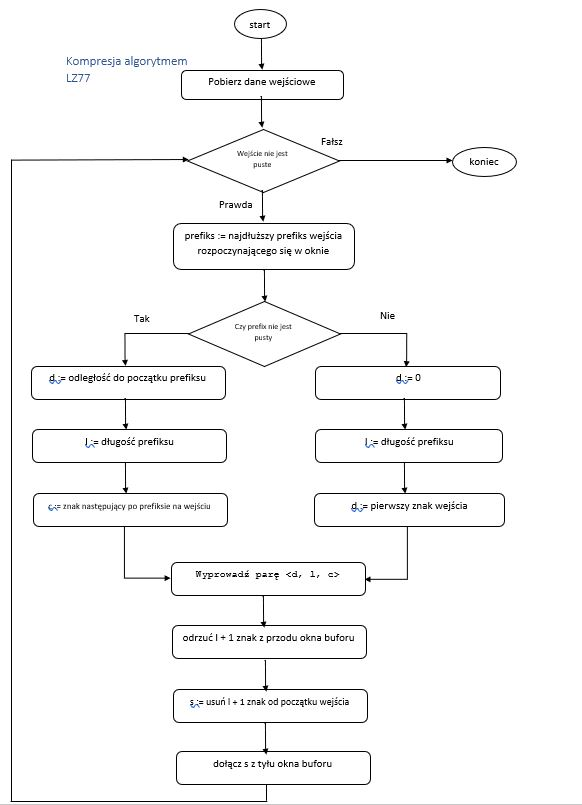
\includegraphics[height=400px]{img/schemat_lz77.JPG}
\end{figure}

\subsubsection{Pseudokod}
\begin{verbatim}
WHILE wejście nie jest puste DO
    prefiks := najdłuższy prefiks wejścia rozpoczynającego się w oknie
    
    IF prefiks nie jest pusty
        d := odległość do początku prefiksu
        l := długość prefiksu
        c := znak następujący po prefiksie na wejściu
    ELSE
        d := 0
        l := 0
        c := pierwszy znak wejścia
    END IF
    
    wyprowadź na wyjście <d, l, c>
    
    odrzuć l + 1 znak z przodu okna buforu
    s := usuń l + 1 znak od początku wejścia
    dołącz s z tyłu okna buforu
REPEAT
\end{verbatim}

\subsubsection{Schemat poglądowy działania na przykładzie - Kodowanie}
Poniżej zaprezentowano sposoby kompresji i dekompresji za pomocą algorytmów Lempel-Ziv (LZ77, \textit{LZ78}), oraz dodatkowo sposób kompresji za pomocą algorytmu Lempel-Ziv-Welch (LZW).
W każdym z przykładów posłużyłem się ciągiem znaków: $aaabbbbbbaaaabbbb$.\\ Dla przykładu ustalamy słownik (lewa strona) i bufor (prawa strona) na 8.
\begin{figure}[h!]
\centering
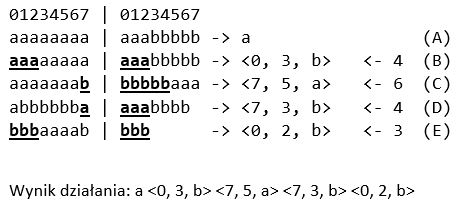
\includegraphics{img/lz77_1.JPG}
\end{figure}

\newpage

\begin{figure}[h!]
\centering
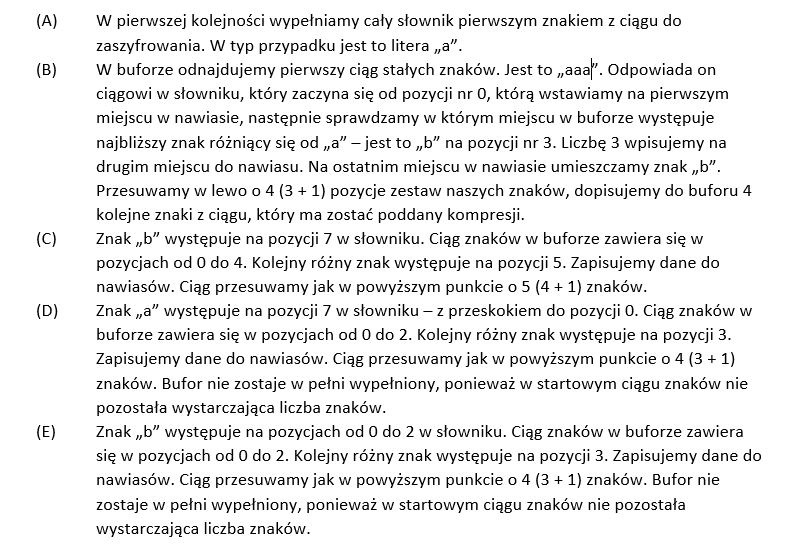
\includegraphics{img/lz77_2.JPG}
\end{figure}

\subsubsection{Schemat poglądowy działania na przykładzie - deKodowanie}
DeKodowanie algorytmów \textit{LZ77} i \textit{LZ78} została umieszczona w sprawozdaniu jako dodatek.\\Dekompresujemy ten sam przykład:

\begin{figure}[h!]
\centering
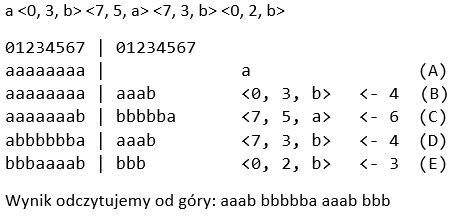
\includegraphics{img/lz77_3.JPG}
\end{figure}

\newpage

\begin{figure}[h!]
\centering
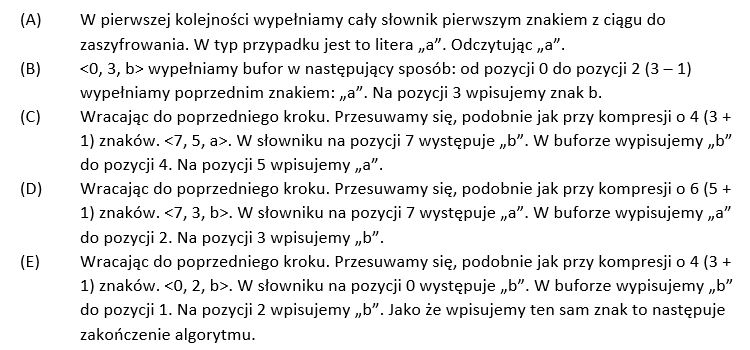
\includegraphics{img/lz77_4.JPG}
\end{figure}

\subsection{LZ78}
W algorytmie \textit{LZ78} pobiera się następne symbole kodowanego ciągu budując z nich pewną frazę. Po pobraniu kolejnego symbolu i dodaniu  go  na końcu już zbudowane  frazy sprawdza się, czy słownik tę frazę zawiera. Jeżeli frazy nie ma w słowniku, to wyprowadzany jest indeks najdłuższej dopasowanej frazy i  ostatnio  pobrany  symbol.  Po  zakodowaniu frazy i symbolu wstawia się do słownika frazę, dla której  operacja szukania zakończyła się niepowodzeniem i rozpoczyna się budowanie nowej frazy od frazy pustej. 

\subsubsection{Schemat blokowy}
\begin{figure}[h!]
\centering
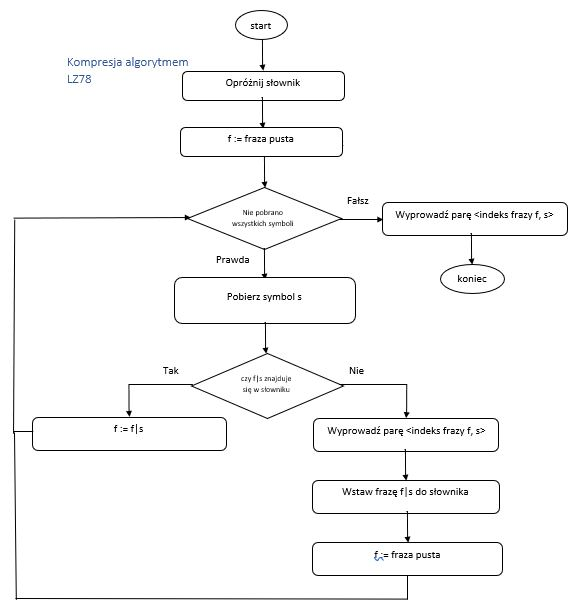
\includegraphics[height=300px]{img/schemat_lz78.JPG}
\end{figure}

\newpage
\subsubsection{Pseudokod}
\begin{verbatim}
opróżnij słownik
f := fraza pusta
WHILE nie pobrano wszystkich symboli komunikatu DO  
    pobierz symbol s
    IF (f|s znajduje się w słowniku)
        f := f|s
    ELSE
        wyprowadź na wyjście <indeks frazy f, s>  
        wstaw frazę f|s do słownika 
        f := fraza pusta
    END IF
END WHILE
wyprowadź na wyjście <indeks frazy f, s>
\end{verbatim}

\subsubsection{Schemat poglądowy działania na przykładzie - Kodowanie}
Dla przypomnienia, posługujemy się następującym ciągiem. $aaabbbbbbaaaabbbb$.

\begin{figure}[h!]
\centering
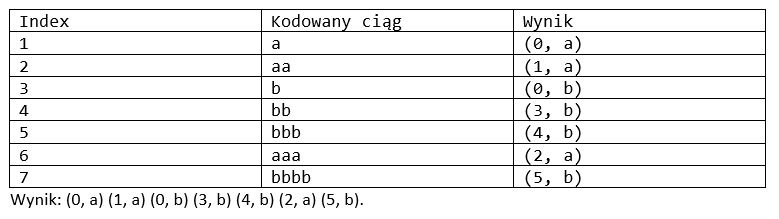
\includegraphics{img/lz78_1.JPG}
\end{figure}

\begin{figure}[h!]
\centering
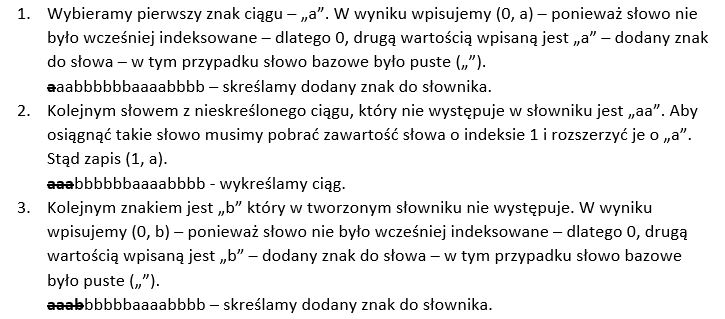
\includegraphics{img/lz78_2.JPG}
\end{figure}

\newpage

\begin{figure}[h!]
\centering
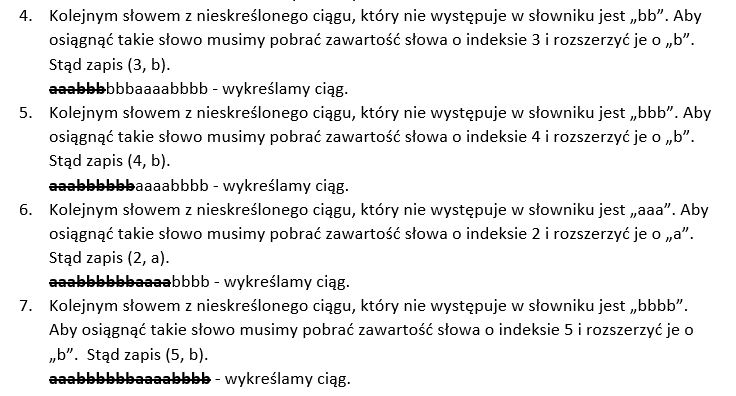
\includegraphics{img/lz78_2_1.JPG}
\end{figure}

\subsubsection{Schemat poglądowy działania na przykładzie - deKodowanie}
\begin{figure}[h!]
\centering
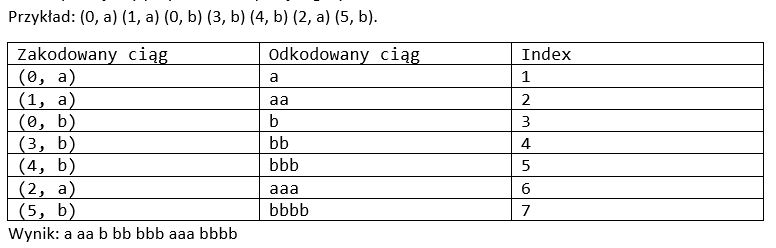
\includegraphics{img/lz78_3.JPG}
\end{figure}

\newpage

\begin{figure}[h!]
\centering
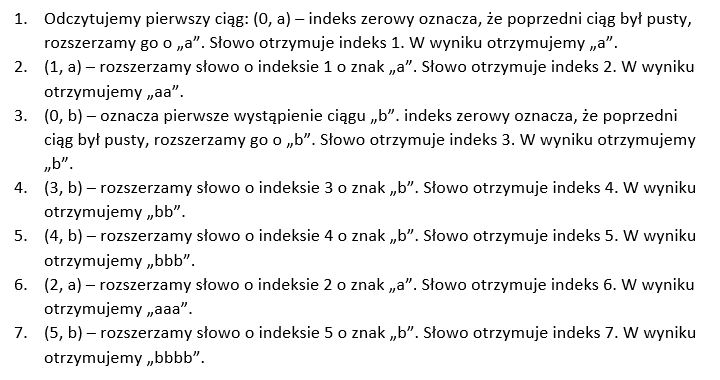
\includegraphics{img/lz78_4.JPG}
\end{figure}

\subsection{LZW}
Algorytm \textit{LZW} jest udoskonaleniem algorytmu \textit{LZ78} polegającym na wstępnym wypełnieniu słownika jednoznakowymi frazami ze wszystkimi symbolami występującymi w alfabecie. Wyprowadzane są tylko indeksy fraz. Współczynniki kompresji \textit{LZW} są lepsze niż w przypadku używania algorytmu \textit{LZ78}.

\subsubsection{Schemat blokowy}
\begin{figure}[h!]
\centering
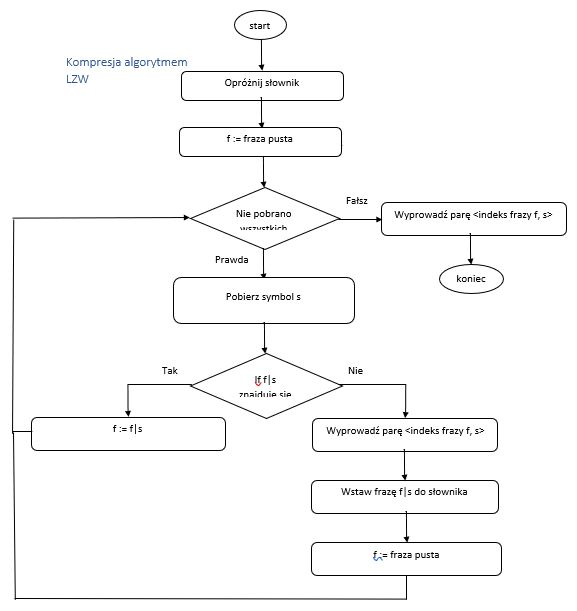
\includegraphics[height=300px]{img/schemat_lzw.JPG}
\end{figure}

\subsubsection{Pseudokod}
\begin{verbatim}
zainicjalizuj słownik
f := fraza pusta
WHILE nie pobrano wszystkich symboli komunikatu DO  
    pobierz symbol s
    IF (f|s znajduje się w słowniku)
        f := f|s
    ELSE
        wyprowadź indeks frazy f
        wstaw frazę f|s do słownika 
        f := s
    END IF
END WHILE
wyprowadź indeksy frazy f
\end{verbatim}

\subsubsection{Schemat poglądowy działania na przykładzie - Kodowanie}
Dla przypomnienia, posługujemy się następującym ciągiem. $aaabbbbbbaaaabbbb$.\\
Algorytm jest bardzo podobny do algorytmu \textit{LZ78} – z tym, że ograniczamy się do indeksów.

\begin{figure}[h!]
\centering
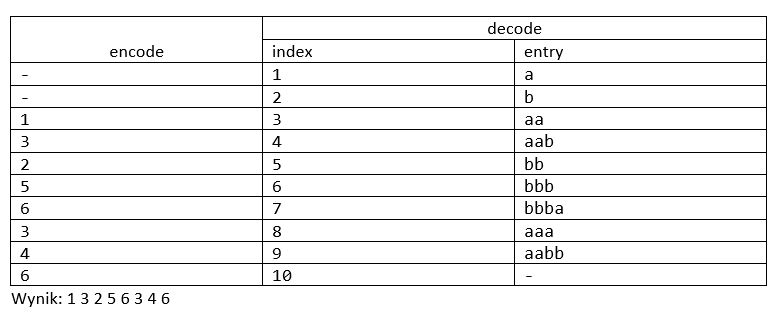
\includegraphics{img/lzw_1.JPG}
\end{figure}

\begin{figure}[h!]
\centering
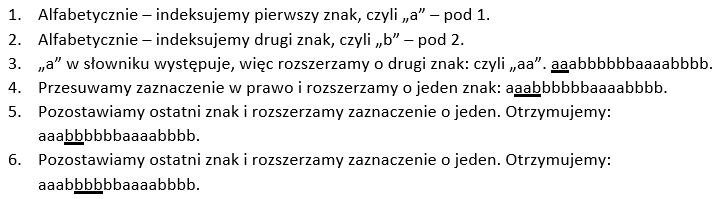
\includegraphics{img/lzw_2.JPG}
\end{figure}

\newpage

\begin{figure}[h!]
\centering
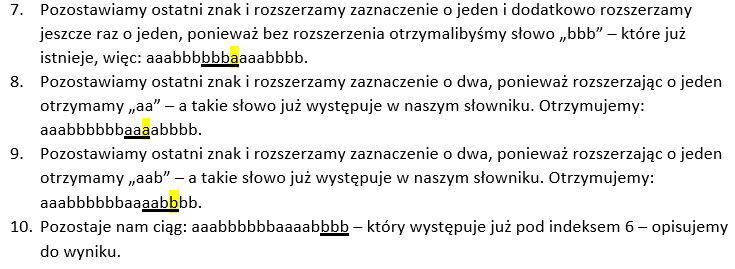
\includegraphics{img/lzw_2_1.JPG}
\end{figure}

\section{Czas wykonywania algorytmów}
Porównane zostały czasy wykonywania kompresji i dekompresji powyższych trzech algorytmów tj.: \textit{LZ77}, \textit{LZ78} i \textit{LZW}. W tym celu wykorzystane zostało narzędzie timera z biblioteki \textit{timeit}. Pierwszy test został przeprowadzony dla ciągu znaków wykorzystywanego w powyższych przykładach, czyli: $aaabbbbbbaaaabbbb$.\\ Drugi test został przeprowadzony dla ciągu:\\ $wszczebrzeszyniechrzaszczbrzmiwtrzcinie$.\\ Wyniki zostały przedstawione poniżej:
\setcounter{figure}{0}
\begin{figure}[h!]
\centering
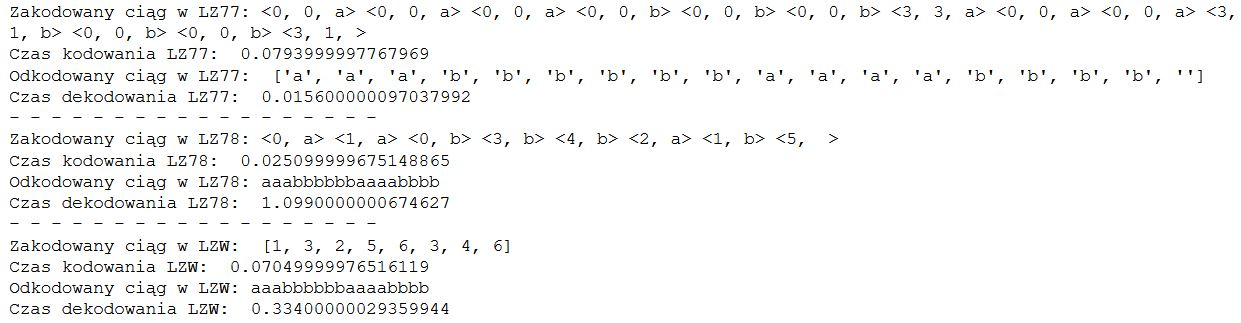
\includegraphics[width=\textwidth]{img/time1.JPG}
\caption{Twórcy algorytmu: Abraham Lempel oraz Jacob Ziv.}
\end{figure}

\begin{figure}[h!]
\centering
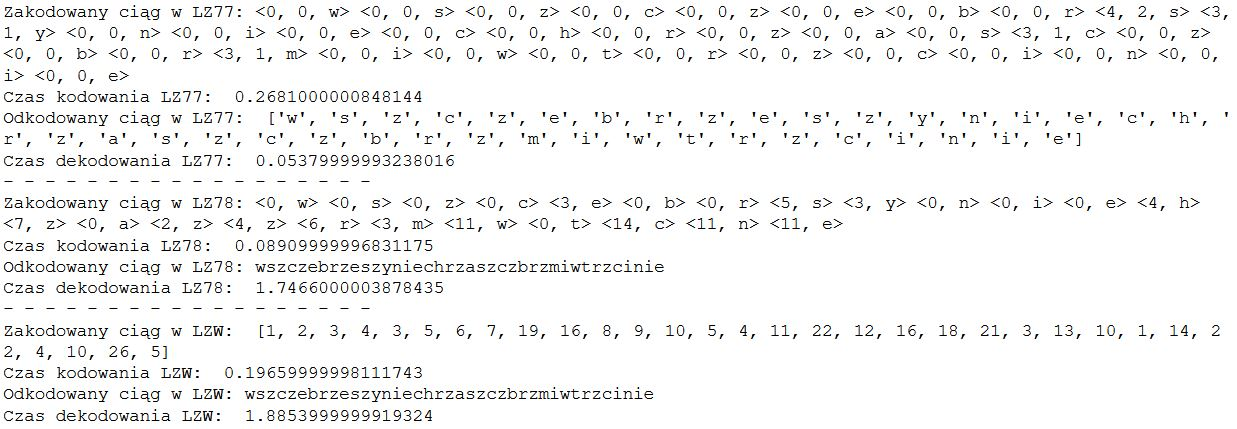
\includegraphics[width=\textwidth]{img/time2.JPG}
\caption{Twórcy algorytmu: Abraham Lempel oraz Jacob Ziv.}
\end{figure}
\newpage

Algorytmy kompresji w kodowaniu \textit{LZ77} jest dużo bardziej złożony niż algorytm dekompresji. W kodowaniu \textit{LZ77} można wpływać bezpośrednio na prędkość kompresji, regulując parametry kodera (rozmiar słownika i bufora kodowania - w teście odpowiednio ustawione na 8 i 6). Stąd możliwe, że najlepsze wyniki w powyższym teście osiągnął właśnie algorytm \textit{LZ77}. Wyniki czasowe działania algorytmów \textit{LZ78} i \textit{LZW} (który tak naprawdę jest wariantem \textit{LZ78}) są bardzo zbliżone do siebie.

\section{Dodatek: ręczne obliczenia}
Zaprezentowane zostały tutaj ręczne obliczenia, które posłużyły do przedstawienia przykładów we wcześniejszych podpunktach.
\subsection{Kodowanie i dekodowanie w \textit{LZ77}}
\begin{figure}[h!]
\centering
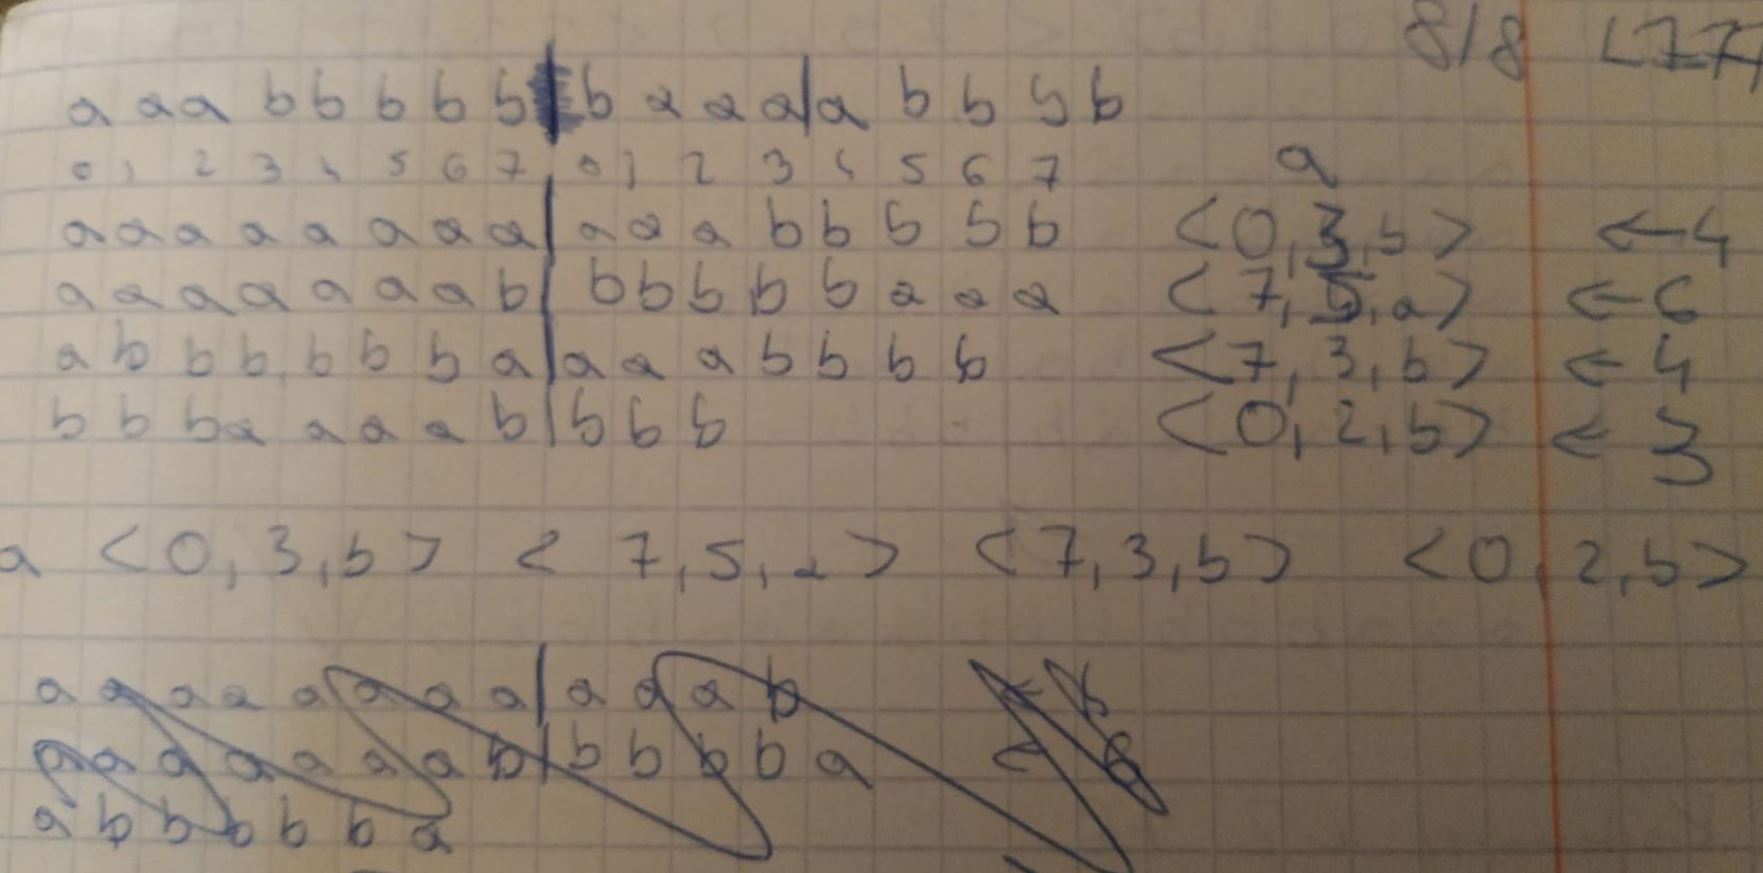
\includegraphics[width=450px]{img/obl_lz77_0.JPG}
\end{figure}

\begin{figure}[h!]
\centering
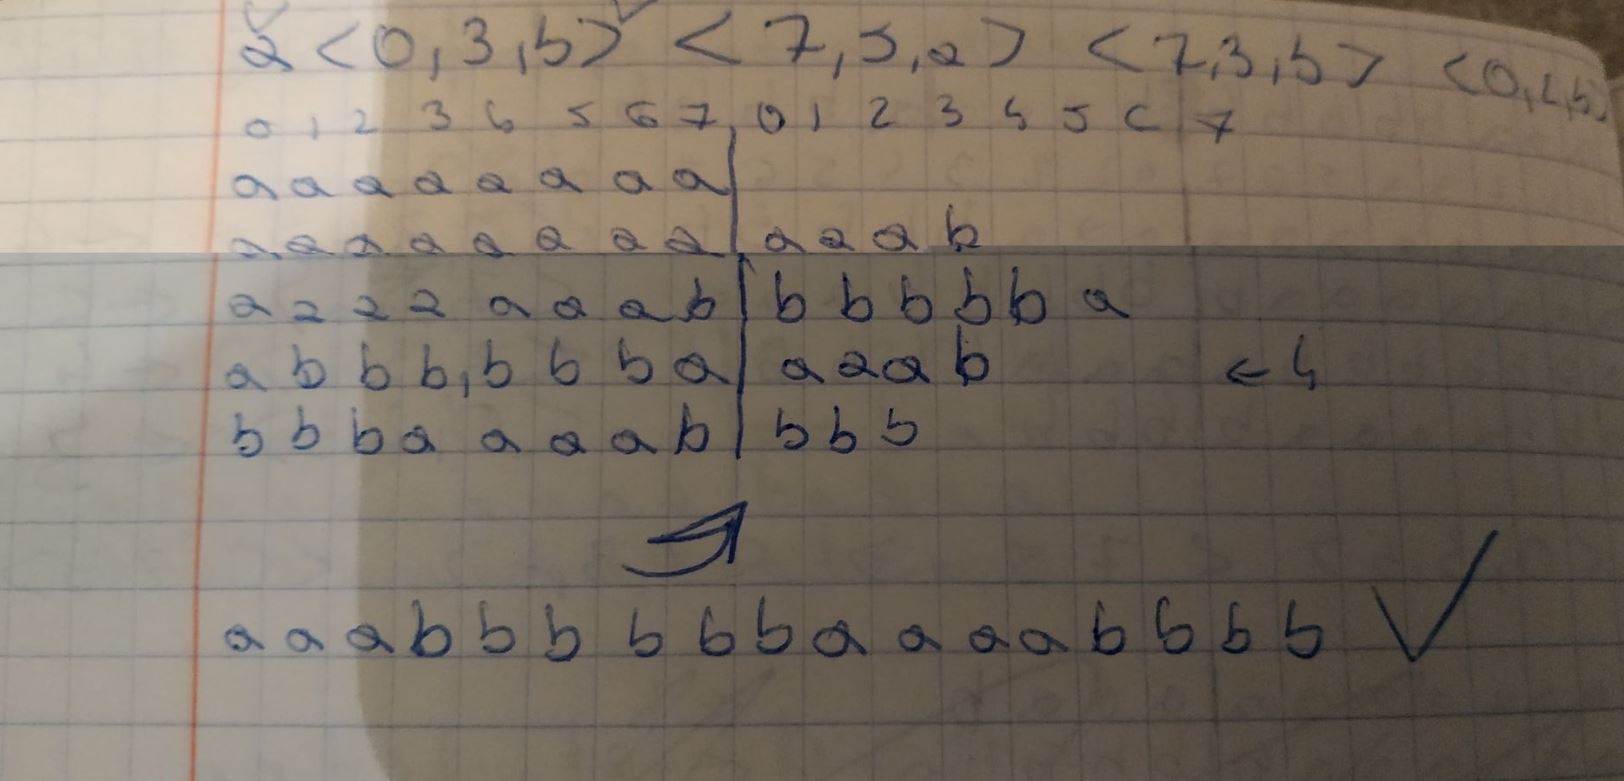
\includegraphics[width=450px]{img/obl_lz77_1.JPG}
\end{figure}

\newpage

\subsection{Kodowanie i dekodowanie w \textit{LZ78}}
\begin{figure}[h!]
\centering
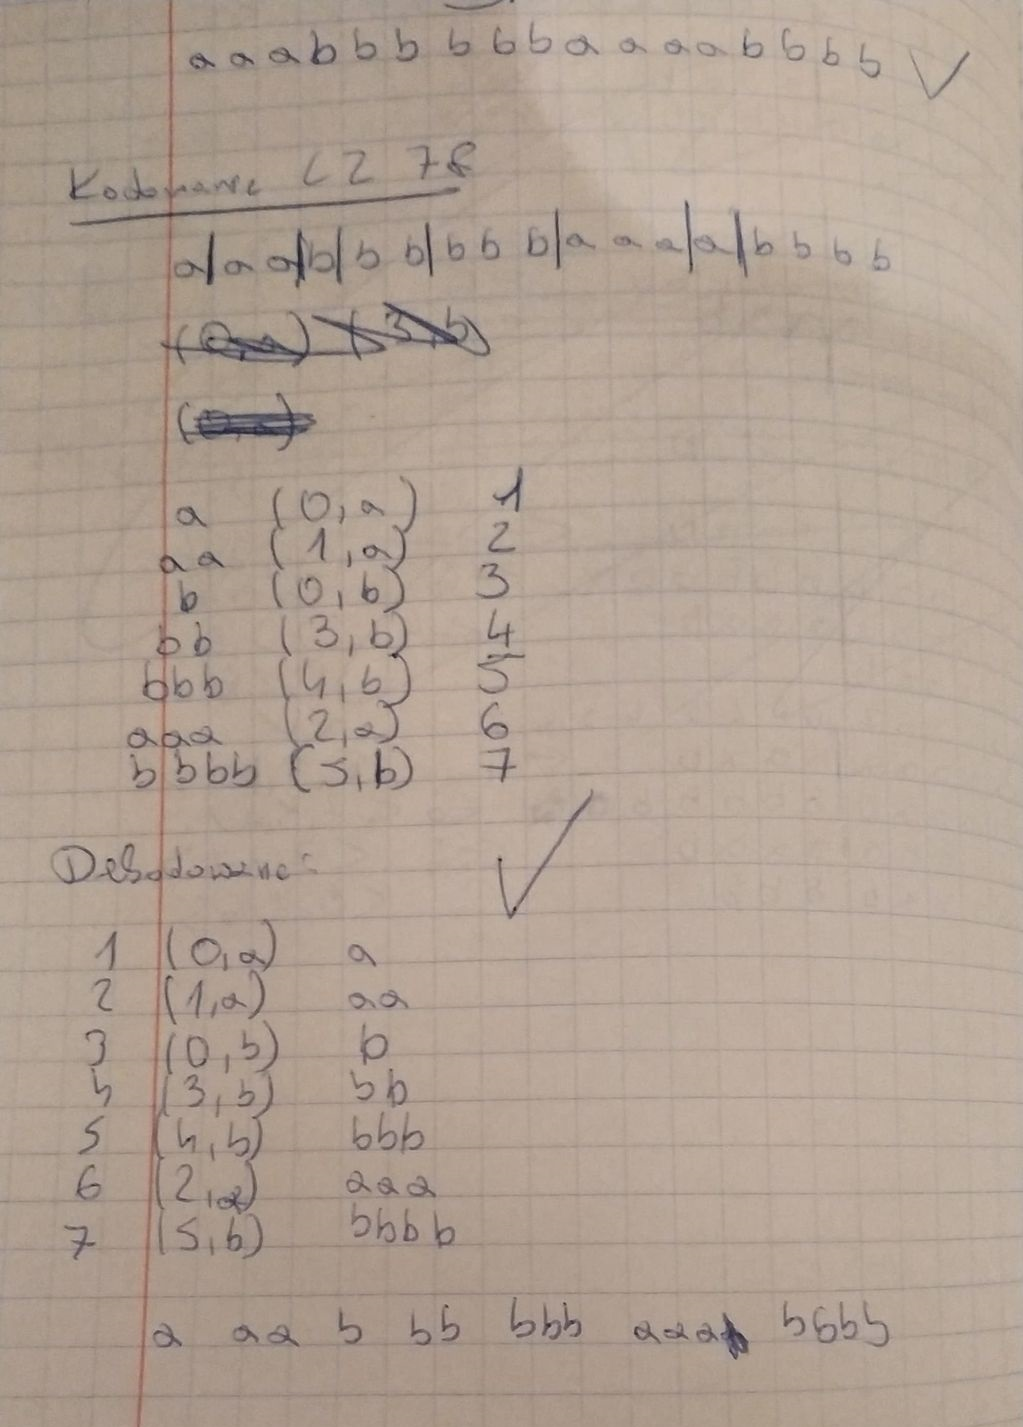
\includegraphics[width=450px]{img/obl_lz78.jpg}
\end{figure}

\newpage

\subsection{Kodowanie w \textit{LZW}}
\begin{figure}[h!]
\centering
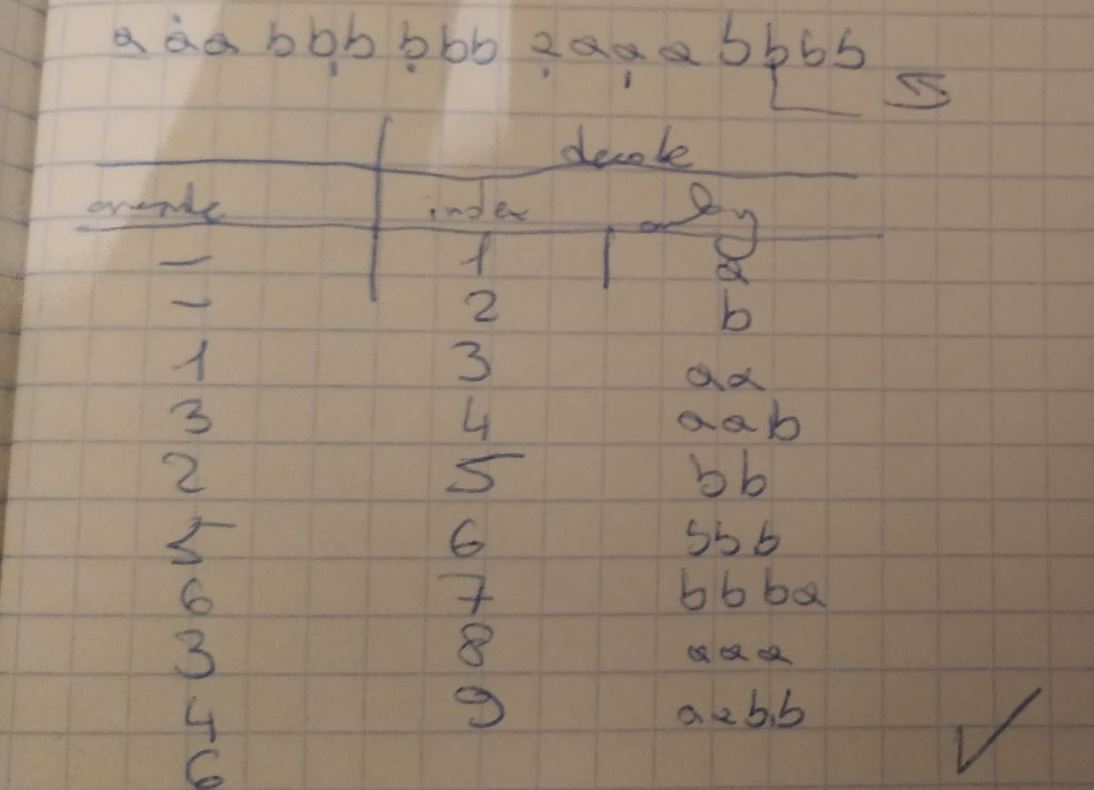
\includegraphics[width=450px]{img/obl_lzw.jpg}
\end{figure}

\textbf{SCHEMATY BLOKOWE I POGLĄDOWE - WRAZ Z OPISEM SĄ DOSTĘPNE W WERSJI DO EDYCJI W ZAŁĄCZONYM DO SPRAWOZDANIA PLIKU .DOCX.}

\begin{thebibliography}{9}
\bibitem{3} 
Drozdek A.: Wprowadzenie do kompresji danych. WNT, Warszawa 1999.
\bibitem{4} 
Starosolski R.: Algorytmy bezstratnej kompresji danych. Studia Informatica, Vol. 24 Number 1(52), Politechnika Śląska 2003.
\bibitem{1} 
Ziv J., Lempel A.: A universal algorithm for sequential data compression. IEEE Transactions on Information Theory, Vol. 32(3), May 1977, pp. 337-43. \bibitem{2} 
Ziv  J.,  Lempel  A.: Compression of individual sequences via variable rate coding. IEEE Transactions on Information Theory, Vol. 24(5), Sept. 1978, pp. 530-6.
\bibitem{5}
Wolfram S. A New Kind of Science. Champaign, IL: Wolfram Media, 2002. 1069.
\bibitem{6}
USPTO Patent no. 4814746. \newline \url{http://www.theregister.co.uk/1999/09/01/unisys_demands_5k_licence_fee} \newline(dostęp 09.06.2021)
\end{thebibliography}

\end{document}